\subsection{Instrumentation Amplifier}

\subsubsection{Circuito con Opamp}

\begin{wrapfigure}[13]{r}{0.5\textwidth}
  \begin{center}
    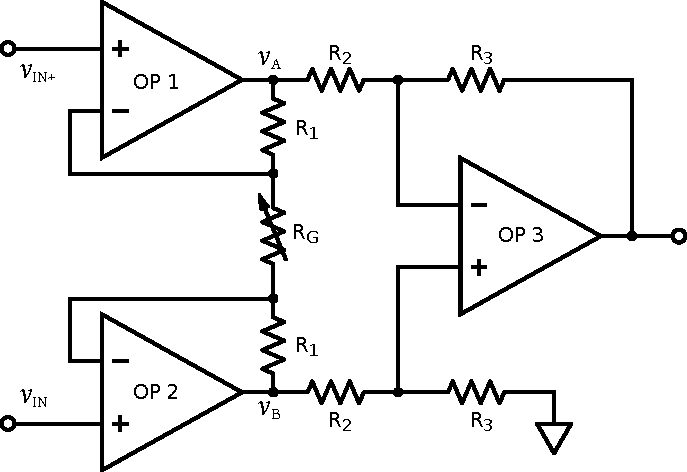
\includegraphics[width=0.350\textwidth]{../E05/latex/c_INA.pdf}
  \end{center}
  \caption{Circuito dell'amplificatore per strumentazione.}
  \label{cir5:instr_amplif}
\end{wrapfigure}

Il circuito visto al paragrafo precedente presenta dei problemi, nonostante abbatta in maniera abbastanza efficiente i segnali di modo comune. Per prima cosa l'impedenza in ingresso vista da un eventuale generatore di segnale è bassa, e ciò rende necessaria una potenza maggiore da parte del generatore per mantenere la tensione ai suoi capi; il secondo luogo, il guadagno non è impostabile (se non cambiando le resistenze ad ogni applicazione: procedura scomoda nelle applicazioni pratiche).

Per ovviare a questi problemi, valutiamo l'amplificatore differenziale in Figura \ref{cir5:instr_amplif}. Si nota subito che l'impedenza in ingresso è molto alta, in quanto gli amplificatori operazionali hanno un valore di impedenza molto alta ai loro ingressi (non a caso sono usati in configurazione follower per adattare le impedenze).

Verifichiamo invece che la resistenza posta in mezzo varia effettivamente il guadagno del circuito. Dividiamo il circuito in due parti, calcolandoci prima la tensione fra il punto A e B\footnote{Si noti che un circuito che abbia come $V_{out}$ la differenza fra questi due punti sarebbe flottante sull'uscita. Infatti, una eventuale resistenza di carico messa fra il punto A e B non avrebbe un riferimento di comune.}, per poi la tensione di uscita dell'intero circuito. Per la prima parte, considerando i due operazionali ideali, otteniamo che le tensione agli ingressi invertenti sono $V_{OP_1}^- = V_1$ e $V_{OP_2}^- = V_2$. Dunque ai capi di $R_g$ è presente una differenza di potenziale $V_2-V_1 = \Delta V_{in}$; per l'idealità degli OPAMP, abbiamo inoltre che la corrente che passa per le resistenze $R_1$ ed $R_g$ sono uguali. Otteniamo dunque, sommando le cadute di potenziale
$$\Delta V_{AB} = \frac{\Delta V_{in}}{R_g} R_g + \frac{\Delta V_{in}}{R_g} R_1 + \frac{\Delta V_{in}}{R_g} R_2$$
cioè
\begin{equation}
\Delta V_{AB} = \Delta V_{in} \left(1+\frac{2R_1}{R_g}\right)
\label{eq5:TEMP_calcoli}
\end{equation}

Valutiamo ora la seconda parte del circuito data da $OP_3$. Per quanto riguarda la tensione all'ingresso non invertente, questa è data da un semplice partitore (non scorre corrente nell'ingresso dell'opamp)
$$V^+=V_B \frac{R_3}{R_3+R_2}$$
All'ingresso non invertente vale invece la legge di Kirkhhoff per i nodi
$$\frac{V_A-V^-}{R_2}+\frac{V_{out}-V^-}{R_3}=0$$
da cui
$$V^-=V_A \frac{R_3}{R_2+R_3} + V_{out} \frac{R_2}{R_2+R_3}$$

Uguagliando $V^-$ e $V^+$ (OPAMP ideale), tenendo conto della (\ref{eq5:TEMP_calcoli}), otteniamo dunque
$$V_{out}=-\Delta V_{in} \left(1+\frac{2R_1}{R_g}\right)\frac{R_3}{R_2}$$
Modificando la resistenza $R_g$ possiamo dunque controllare il guadagno del circuito.

\subsubsection{Integrato AD622}

\begin{wrapfigure}[13]{r}{0.5\textwidth}
  \begin{center}
    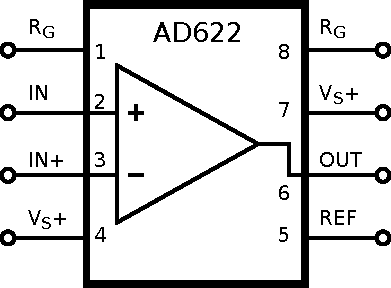
\includegraphics[width=0.260\textwidth]{../E05/latex/AD622.pdf}
  \end{center}
  \caption{Piedinatura dell'integrato AD622.}
  \label{cir5:ad622_piedinatura}
\end{wrapfigure}

In realtà, nell'esperienza abbiamo utilizzato un circuito integrato (più precisamente l'AD622, la cui piedinatura è esposta in Figura \ref{cir5:ad622_piedinatura}) che ha come qualità il fatto di avere un'alta precisione sul valore delle resistenze (abbiamo visto nel precedente circuito che uno squilibrio anche minimo fra i valori di resistenze che dovrebbero essere uguali può portare ad un guadagno diverso da quello teorico). Il suo guadagno è dato dall'equazione, fornita dal costruttore
$$G=1+\frac{50.5 \si{\kilo\ohm}}{R_g}$$

Una possibile applicazione di questo integrato è di utilizzarlo per individuare variazioni di tensione all'interno di un ponte di resistenze. Allo scopo, utilizziamo il circuito in Figura \ref{cir5:ad622_ponte}, con l'accortezza di portare una resistenza del ponte lontana dalle altre, così da poter modificarne la temperatura senza influenzare anche le altre. Infatti, sappiamo che le resistenze hanno una dipendenza dalla temperatura data dal coefficiente di temperatura, che è di circa $200$ ppm/\si{\celsius}. Nel nostro caso, utilizzando come resistenza lontana dalle una da $100$ \si{\ohm}, la sua variazione per grado di temperatura sarà di $\Delta R = 100 \si{\ohm} (-200 \times 10^{-6}) = -20$ \si{\milli\ohm/\celsius}. Inoltre, per il ponte vale che non vi è differenza di tensione fra gli ingressi dell'integrato se il prodotto delle resistenze $R_1 R_4=R_2 R_3$: dunque, variando la resistenza $R_3$ inizieremo a registrare una tensione di uscita.

\begin{wrapfigure}[13]{r}{0.5\textwidth}
  \begin{center}
    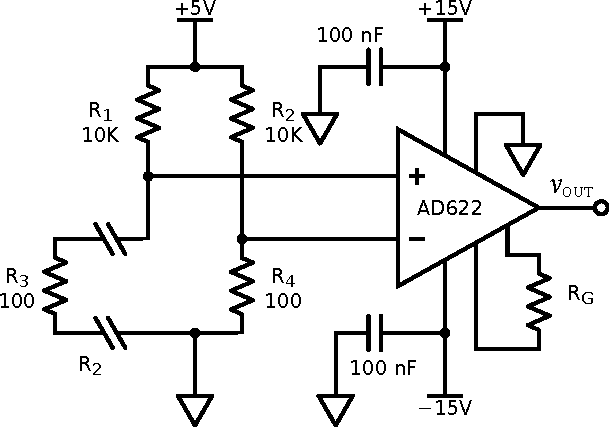
\includegraphics[width=0.260\textwidth]{../E05/latex/c_func_INA.pdf}
  \end{center}
  \caption{Piedinatura dell'integrato AD622.}
  \label{cir5:ad622_ponte}
\end{wrapfigure}

Sperimentalmente, si osserva però che una differenza di potenziale è già presente a temperatura ambiente (cioè senza variare la temperatura della resistenza $R_3$): questo fatto è imputabile al mancato bilanciamento del ponte. Infatti, è impossibile trovare due resistenze che abbiano un valore esattamente identico: dunque vi è un errore sistematico di cui dobbiamo tenere conto prima di effettuare le misure, fissando un valore zero di tensione, che si osserva essere $0.54$\si{\volt}.

Considerando lo zero come sopra, gli altri due valori osservati sono stati di $0.08$ \si{\volt} soffiando sopra la resistenza, e $-0.44$ \si{\volt} con la bomboletta refrigerante.

La relazione che lega la variazione di tensione alla resistenza è
$$\Delta V = A \frac{\Delta R}{R + R_t} V_{b}$$
dove $V_{b}$ è la tensione di alimentazione del ponte (come in Figura \ref{cir5:ad622_ponte}), A il guadagno dell'AD622.